\documentclass[letterpaper, 12pt]{article}
\usepackage[top=2cm,bottom=1cm,left=0.75in,right=0.75in,headheight=17pt, % as per the warning by fancyhdr
includehead,includefoot,
heightrounded, % to avoid spurious underfull messages
]{geometry}
\addtolength{\topmargin}{-.25in}
\usepackage{fancyhdr}
\pagestyle{fancy}
\usepackage{graphicx}
\usepackage{lastpage}
\usepackage{gensymb}

\begin{document}
\fancyhead[l]{	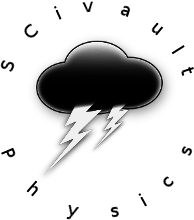
\includegraphics[height=1.2cm]{../Logo/sp.png} Name:}
\fancyhead[r]{REFERENCE MATERIAL}
\cfoot{\thepage\ of \pageref{LastPage}}
	


\begin{center}Things to Memorize: Newton's Laws
\end{center}


\subsection*{Force}
\begin{itemize}
	\item A \textbf{Force} is push or a pull on something. 
	\item Force is a Vector.  It is symbolized by the symbol $\vec{F}$
	\item Force is measured in kg m/s\textsuperscript{2}.  This is often abbreviated as N (newtons).  
\end{itemize}
\subsection*{Newton's First Law}
\begin{center}
	\textit{Objects in motion will stay in motion and objects at rest will stay at rest until acted on by an external, unbalanced force.}
\end{center}

\begin{itemize}
	\item This means that if there are no forces acting on an object, it will continue to move in the same way it was moving initially - either at rest or in a straight line at a constant speed.
	\item In order for an object to remain at rest, all the forces must be balanced.
	\item In order for an object to travel with constant velocity, all the forces must be balanced.
	
\end{itemize}

\subsection*{Newton's Second Law}
\begin{center}
	\textit{The acceleration of an object as produced by a net force is directly proportional to the magnitude of the net force, in the same direction as the net force, and inversely proportional to the mass of the object.}
\end{center}
	\begin{itemize}
	\item This is often written as a formula: $ \Sigma\vec{F} = m \vec{a}$ or $ \vec{F_{net}} = m \vec{a}$
	\item If an object is accelerating, there must be at least one unbalanced force acting on the object. 
	\item The first law is just a special case of the second law: If the net force acting on an object is zero, its acceleration will be zero. 
\end{itemize}





 

\subsection*{Newton's Third Law}
\begin{center}
	\textit{For every action there is an equal and opposite reaction.}
\end{center}
\begin{itemize}
	\item The action and reaction pairs are always simultaneous.
	\item The action and reaction pairs are always the same in magnitude.
	\item The action and reaction paris are always in opposite directions.
	
\end{itemize}

\subsection*{Mass and Weight}
	\begin{itemize}
		\item The \textbf{mass} of an object measures how much matter an object is made of.  It is measured in kilograms.
		\item The \textbf{weight} of an object is a force due to gravity. It is measured in newtons.
		
	\end{itemize}

\subsection*{Friction}
\begin{itemize}
	\item Friction is a force that opposes motion or even the tendency to move.
	\item Friction comes in two types:
	\begin{itemize}
		\item \textbf{Static} friction is present when an object is at rest relative to the surface it is on.
		\begin{itemize}
			\item A wheel that is rolling has static friction where it contacts the ground. 
		\end{itemize}
		\item \textbf{Kinetic} friction is present when an object is sliding across a surface.  
	\end{itemize}
	\item The \textbf{maximum static friction} is always greater than or equal to the \textbf{kinetic friction}.
	\item The \textbf{Coefficient of Friction} measures how hard it is for two surfaces to slide past each other. 
	\begin{itemize}
		\item Most coefficients of friction are between 0 and 1, but certain specially-made materials can be much higher.
		\item A \textbf{low} coefficient of friction indicates a slippery surface.
		\item A \textbf{high} coefficient of friction indicates a surface that is very hard to slide on. 
	\end{itemize} 
	
\end{itemize}
 



\end{document}
